% Options for packages loaded elsewhere
\PassOptionsToPackage{unicode}{hyperref}
\PassOptionsToPackage{hyphens}{url}
%
\documentclass[
  stu]{apa7}
\usepackage{amsmath,amssymb}
\usepackage{iftex}
\ifPDFTeX
  \usepackage[T1]{fontenc}
  \usepackage[utf8]{inputenc}
  \usepackage{textcomp} % provide euro and other symbols
\else % if luatex or xetex
  \usepackage{unicode-math} % this also loads fontspec
  \defaultfontfeatures{Scale=MatchLowercase}
  \defaultfontfeatures[\rmfamily]{Ligatures=TeX,Scale=1}
\fi
\usepackage{lmodern}
\ifPDFTeX\else
  % xetex/luatex font selection
\fi
% Use upquote if available, for straight quotes in verbatim environments
\IfFileExists{upquote.sty}{\usepackage{upquote}}{}
\IfFileExists{microtype.sty}{% use microtype if available
  \usepackage[]{microtype}
  \UseMicrotypeSet[protrusion]{basicmath} % disable protrusion for tt fonts
}{}
\makeatletter
\@ifundefined{KOMAClassName}{% if non-KOMA class
  \IfFileExists{parskip.sty}{%
    \usepackage{parskip}
  }{% else
    \setlength{\parindent}{0pt}
    \setlength{\parskip}{6pt plus 2pt minus 1pt}}
}{% if KOMA class
  \KOMAoptions{parskip=half}}
\makeatother
\usepackage{xcolor}
\usepackage{graphicx}
\makeatletter
\def\maxwidth{\ifdim\Gin@nat@width>\linewidth\linewidth\else\Gin@nat@width\fi}
\def\maxheight{\ifdim\Gin@nat@height>\textheight\textheight\else\Gin@nat@height\fi}
\makeatother
% Scale images if necessary, so that they will not overflow the page
% margins by default, and it is still possible to overwrite the defaults
% using explicit options in \includegraphics[width, height, ...]{}
\setkeys{Gin}{width=\maxwidth,height=\maxheight,keepaspectratio}
% Set default figure placement to htbp
\makeatletter
\def\fps@figure{htbp}
\makeatother
\setlength{\emergencystretch}{3em} % prevent overfull lines
\providecommand{\tightlist}{%
  \setlength{\itemsep}{0pt}\setlength{\parskip}{0pt}}
\setcounter{secnumdepth}{-\maxdimen} % remove section numbering
% Make \paragraph and \subparagraph free-standing
\ifx\paragraph\undefined\else
  \let\oldparagraph\paragraph
  \renewcommand{\paragraph}[1]{\oldparagraph{#1}\mbox{}}
\fi
\ifx\subparagraph\undefined\else
  \let\oldsubparagraph\subparagraph
  \renewcommand{\subparagraph}[1]{\oldsubparagraph{#1}\mbox{}}
\fi
% definitions for citeproc citations
\NewDocumentCommand\citeproctext{}{}
\NewDocumentCommand\citeproc{mm}{%
  \begingroup\def\citeproctext{#2}\cite{#1}\endgroup}
\makeatletter
 % allow citations to break across lines
 \let\@cite@ofmt\@firstofone
 % avoid brackets around text for \cite:
 \def\@biblabel#1{}
 \def\@cite#1#2{{#1\if@tempswa , #2\fi}}
\makeatother
\newlength{\cslhangindent}
\setlength{\cslhangindent}{1.5em}
\newlength{\csllabelwidth}
\setlength{\csllabelwidth}{3em}
\newenvironment{CSLReferences}[2] % #1 hanging-indent, #2 entry-spacing
 {\begin{list}{}{%
  \setlength{\itemindent}{0pt}
  \setlength{\leftmargin}{0pt}
  \setlength{\parsep}{0pt}
  % turn on hanging indent if param 1 is 1
  \ifodd #1
   \setlength{\leftmargin}{\cslhangindent}
   \setlength{\itemindent}{-1\cslhangindent}
  \fi
  % set entry spacing
  \setlength{\itemsep}{#2\baselineskip}}}
 {\end{list}}
\usepackage{calc}
\newcommand{\CSLBlock}[1]{\hfill\break\parbox[t]{\linewidth}{\strut\ignorespaces#1\strut}}
\newcommand{\CSLLeftMargin}[1]{\parbox[t]{\csllabelwidth}{\strut#1\strut}}
\newcommand{\CSLRightInline}[1]{\parbox[t]{\linewidth - \csllabelwidth}{\strut#1\strut}}
\newcommand{\CSLIndent}[1]{\hspace{\cslhangindent}#1}
\ifLuaTeX
\usepackage[bidi=basic]{babel}
\else
\usepackage[bidi=default]{babel}
\fi
\babelprovide[main,import]{british}
% get rid of language-specific shorthands (see #6817):
\let\LanguageShortHands\languageshorthands
\def\languageshorthands#1{}
% Manuscript styling
\usepackage{upgreek}
\captionsetup{font=singlespacing,justification=justified}

% Table formatting
\usepackage{longtable}
\usepackage{lscape}
% \usepackage[counterclockwise]{rotating}   % Landscape page setup for large tables
\usepackage{multirow}		% Table styling
\usepackage{tabularx}		% Control Column width
\usepackage[flushleft]{threeparttable}	% Allows for three part tables with a specified notes section
\usepackage{threeparttablex}            % Lets threeparttable work with longtable

% Create new environments so endfloat can handle them
% \newenvironment{ltable}
%   {\begin{landscape}\centering\begin{threeparttable}}
%   {\end{threeparttable}\end{landscape}}
\newenvironment{lltable}{\begin{landscape}\centering\begin{ThreePartTable}}{\end{ThreePartTable}\end{landscape}}

% Enables adjusting longtable caption width to table width
% Solution found at http://golatex.de/longtable-mit-caption-so-breit-wie-die-tabelle-t15767.html
\makeatletter
\newcommand\LastLTentrywidth{1em}
\newlength\longtablewidth
\setlength{\longtablewidth}{1in}
\newcommand{\getlongtablewidth}{\begingroup \ifcsname LT@\roman{LT@tables}\endcsname \global\longtablewidth=0pt \renewcommand{\LT@entry}[2]{\global\advance\longtablewidth by ##2\relax\gdef\LastLTentrywidth{##2}}\@nameuse{LT@\roman{LT@tables}} \fi \endgroup}

% \setlength{\parindent}{0.5in}
% \setlength{\parskip}{0pt plus 0pt minus 0pt}

% Overwrite redefinition of paragraph and subparagraph by the default LaTeX template
% See https://github.com/crsh/papaja/issues/292
\makeatletter
\renewcommand{\paragraph}{\@startsection{paragraph}{4}{\parindent}%
  {0\baselineskip \@plus 0.2ex \@minus 0.2ex}%
  {-1em}%
  {\normalfont\normalsize\bfseries\itshape\typesectitle}}

\renewcommand{\subparagraph}[1]{\@startsection{subparagraph}{5}{1em}%
  {0\baselineskip \@plus 0.2ex \@minus 0.2ex}%
  {-\z@\relax}%
  {\normalfont\normalsize\itshape\hspace{\parindent}{#1}\textit{\addperi}}{\relax}}
\makeatother

\makeatletter
\usepackage{etoolbox}
\patchcmd{\maketitle}
  {\section{\normalfont\normalsize\abstractname}}
  {\section*{\normalfont\normalsize\abstractname}}
  {}{\typeout{Failed to patch abstract.}}
\patchcmd{\maketitle}
  {\section{\protect\normalfont{\@title}}}
  {\section*{\protect\normalfont{\@title}}}
  {}{\typeout{Failed to patch title.}}
\makeatother

\usepackage{xpatch}
\makeatletter
\xapptocmd\appendix
  {\xapptocmd\section
    {\addcontentsline{toc}{section}{\appendixname\ifoneappendix\else~\theappendix\fi\\: #1}}
    {}{\InnerPatchFailed}%
  }
{}{\PatchFailed}
\keywords{keywords\newline\indent Word count: X}
\usepackage{csquotes}
\usepackage[titles]{tocloft}
\cftpagenumbersoff{figure}
\renewcommand{\cftfigpresnum}{\itshape\figurename\enspace}
\renewcommand{\cftfigaftersnum}{.\space}
\setlength{\cftfigindent}{0pt}
\setlength{\cftafterloftitleskip}{0pt}
\settowidth{\cftfignumwidth}{Figure 10.\qquad}
\cftpagenumbersoff{table}
\renewcommand{\cfttabpresnum}{\itshape\tablename\enspace}
\renewcommand{\cfttabaftersnum}{.\space}
\setlength{\cfttabindent}{0pt}
\setlength{\cftafterloftitleskip}{0pt}
\settowidth{\cfttabnumwidth}{Table 10.\qquad}
\makeatletter
\renewcommand{\paragraph}{\@startsection{paragraph}{4}{\parindent}%
  {0\baselineskip \@plus 0.2ex \@minus 0.2ex}%
  {-1em}%
  {\normalfont\normalsize\bfseries\typesectitle}}

\renewcommand{\subparagraph}[1]{\@startsection{subparagraph}{5}{1em}%
  {0\baselineskip \@plus 0.2ex \@minus 0.2ex}%
  {-\z@\relax}%
  {\normalfont\normalsize\bfseries\itshape\hspace{\parindent}{#1}\textit{\addperi}}{\relax}}
\makeatother
\setlength{\cslhangindent}{0.5in}
\usepackage{fancyhdr} 
\pagestyle{fancy}   
\fancyhf{} 
\fancyhead[R]{\thepage} 
\renewcommand{\headrulewidth}{0pt}
\thispagestyle{fancy}
\duedate{07.08.2023}
\course{Modul 6b: Empirisch-Experimentelles Praktikum}
\professor{Dr. Sarina Schäfer}

\ifLuaTeX
  \usepackage{selnolig}  % disable illegal ligatures
\fi
\usepackage{bookmark}
\IfFileExists{xurl.sty}{\usepackage{xurl}}{} % add URL line breaks if available
\urlstyle{same}
\hypersetup{
  pdftitle={The title},
  pdfauthor={First Author1 \& Ernst-August Doelle1,2},
  pdflang={en-GB},
  pdfkeywords={keywords},
  hidelinks,
  pdfcreator={LaTeX via pandoc}}

\title{The title}
\author{First Author\textsuperscript{1} \& Ernst-August Doelle\textsuperscript{1,2}}
\date{}


\shorttitle{Title}

\authornote{

Add complete departmental affiliations for each author here. Each new line herein must be indented, like this line.

Enter author note here.

The authors made the following contributions. First Author: Conceptualization, Writing - Original Draft Preparation, Writing - Review \& Editing; Ernst-August Doelle: Writing - Review \& Editing, Supervision.

Correspondence concerning this article should be addressed to First Author, Postal address. E-mail: \href{mailto:my@email.com}{\nolinkurl{my@email.com}}

}

\affiliation{\vspace{0.5cm}\textsuperscript{1} Wilhelm-Wundt-University\\\textsuperscript{2} Konstanz Business School}

\note{\clearpage}

\abstract{%
One or two sentences providing a \textbf{basic introduction} to the field, comprehensible to a scientist in any discipline.
Two to three sentences of \textbf{more detailed background}, comprehensible to scientists in related disciplines.
One sentence clearly stating the \textbf{general problem} being addressed by this particular study.
One sentence summarizing the main result (with the words ``\textbf{here we show}'' or their equivalent).
Two or three sentences explaining what the \textbf{main result} reveals in direct comparison to what was thought to be the case previously, or how the main result adds to previous knowledge.
One or two sentences to put the results into a more \textbf{general context}.
Two or three sentences to provide a \textbf{broader perspective}, readily comprehensible to a scientist in any discipline.
}



\begin{document}
\maketitle

\section{Methods}\label{methods}

\subsection{Preregistration and version control}\label{preregistration-and-version-control}

The hypotheses, the inclusion/exclusion criteria, used databases, search queries and the basic theoretical foundation of this systematic literature review are preregistered and can be found on Moodle or in the GitHub repository.\\
As suggested by Lakens (2022) (Chapter 14), the present systemic literature used a GitHub repository to store all data and files. The repository is available at: \url{https://github.com/julianrottenberg/Stereotype_Threat_im_akademischen_Kontext}\\
This approach allows for more transparency and reproducibility as well as accountability.

\subsection{Artificial Intelligence (AI)}\label{artificial-intelligence-ai}

It should be acknowledged that artificial intelligence has been used as an aid in this review - namely, Anthropic's Claude AI 3.5 Sonnet (Anthropic, 2024) and GitHub's Copilot (GitHub \& OpenAi, 2024), the latter was directly integrated into RStudio Server (Posit team, 2024). The chats that directly influenced this review are all available on the GitHub repository.
For Github Copilot the autocomplete-style suggestions were used.\\
Claude AI 3.5 Sonnet was used to generate descriptions of the papers used in this review - based on a template.
The process here was as follows: First the template was manually filled out by a human, after this process was completed for every paper, a second template was created, the contents of which were filled out by AI and then, later, used in conjunction with the manually created templates. When the different templates differed from one another the primary source (i.e.~the paper the template was based on) was checked again. Both, the human-generated as well as the AI-generated templates can be found on the GitHub repository - the AI generated summaries have been marked as such, beginning with ``Claude\_Ai\_'' in their file name.\\
To clarify, AI was not used to generate any of the text in this review, it was used as a tool to gather a better understanding and overview of the papers involved. The process of having a human and AI created summary of each paper was chosen to gather an extra layer of security regarding the contents of each paper as well as to counteract possible oversights.

\subsection{Identification of relevant papers}\label{identification-of-relevant-papers}

Papers were selected following the criteria outlined in the preregistration:

\subsubsection{Databases, search queries and inclusion/exclusion criteria}\label{databases-search-queries-and-inclusionexclusion-criteria}

The databases used were Web of Science, Google Scholar, PSYNDEX, ResearchRabbit and EBSCOhost Within EBSCOhost, the databases APA PsycArticles, APA PsycInfo, Psychology and Behavioral Sciences Collection, PSYNDEX Literature with PSYNDEX Tests, Education Source Ultimate, and Academic Search Ultimate were searched.\\
Furthermore, the snowball method was utilised to find additional papers - however, this approach did not deliver any additional papers, the same applies to ResearchRabbit.\\
The permalinks to each search used can also be found within the GitHub repository.\\
Within Web of Science the included document types were ``Article'', ``Other'', or ``Clinical Trail''; the excluded document types were ``Book'', ``Meeting'', ``Editorial Material'', or ``Review Article''.
Furthermore, the database ``Preprint Citation Index'' was excluded.\\
In EBSCOhost, ``Apply equivalent subjects'' was applied as an Expander, while ``Peer Reviewed'', ``Document Type*'', and ``Publication Type*'' were used as Limiters.\\
In Google Scholar, the following was added at the end of the search query: ``AND''empirical study'' AND ``peer-reviewed'' -books -meta-analysis)``.\\
These extra filters were applied in accordance with the inclusion and exclusion criteria outlined in the preregistration. No other changes were made to the search queries. An overview of the search queries can be found in Table 1.

\begin{table}[tbp]

\begin{center}
\begin{threeparttable}

\caption{\label{tab:unnamed-chunk-1}Search queries used for the systematic literature review.}

\begin{tabular}{m{4cm}m{12cm}}
\toprule
Hypothesis & \multicolumn{1}{c}{Search Query}\\
\midrule
H1 & ("stereotype threat") AND 
(neural OR neuroimaging OR "functional magnetic resonance imaging" OR fMRI OR electroencephalo* OR EEG OR ERP OR "brain activation" OR amygdala OR "prefrontal cortex" OR "default mode network" OR "salience network") AND
(academ* OR education* OR stud* OR learn* OR perform* OR school OR university OR college)\\
H2 & ("stereotype threat") AND 
("cognitive control" OR "executive function" OR "executive function network" OR "cognitive control network" OR "brain activation" OR "brain activation patterns" OR "cognitive tasks" OR "executive tasks" OR "cognitive assessment" OR "executive assessment") AND 
(academ* OR education* OR stud* OR learn* OR perform* OR school OR university OR college)\\
H3 & ("stereotype threat") AND 
("working memory*" OR "processing speed" OR accuracy) AND 
(academ* OR education* OR stud* OR learn* OR perform* OR school OR university OR college)\\
\bottomrule
\addlinespace
\end{tabular}

\begin{tablenotes}[para]
\normalsize{\textit{Note.} The search queries were used in the databases Web of Science, Google Scholar, PSYNDEX, ResearchRabbit, and EBSCOhost. The permalinks to each search used can be found within the GitHub repository.}
\end{tablenotes}

\end{threeparttable}
\end{center}

\end{table}

The inclusion and exclusion criteria specified in the preregistration were applied to each paper.
The criteria ``Stereotype Threat'', which required studies to ``explicitly examine, manipulate, or measure stereotype threat as a key study variable or factor'' was enforced on a lot of papers and resulted in their exclusion - even when they were otherwise relevant (more on this in the discussion section), same applies to the ``Outcomes'' criteria, which required studies to report ``at least one of the following: 1. Neural activation patterns/brain imaging data; 2. Cognitive processes (e.g., working memory, cognitive control/executive functions)'' also resulted in the exclusion of papers which indirectly measured these outcomes but/or did not specifically focus on ``working memory'' for example - as an example: a paper might have used a test that is known to measure working memory but did not mention ``working memory'' within its abstract, methods or results section, so it was excluded.

\subsubsection{Screening}\label{screening}

The screening process was done using the software Rayyan (Ouzzani et al., 2016). All results were imported onto the platform.
The total amount of papers found was 599 (\(n_{\text{EBSCOhost}} = 105\), \(n_{\text{Google Scholar}} = 48\), \(n_{\text{PSYNDEX}} = 5\), \(n_{\text{ResearchRabbit}} = 4\), \(n_{\text{Web of Science}} = 437\)). Out of these 83 were duplicates (88 were automatically detected by Rayyan, however, 5 were false positives), leaving 516 papers to be screened. During the first screening another 440 papers were excluded.
Papers which were excluded did not fit the inclusion criteria, most prominently, they either did not focus on stereotype threat, had the wrong population (e.g., older adults), did not fit the publication type requirements, or did not measure the outcomes of interest - this was assessed using the title, keywords, and abstract. If neither the title, nor the keywords or abstract mentioned enough information to make a decision, the paper was marked as 'maybe.
An example for hypothesis 3 would be, a paper measured working memory but just referred to ``the participants'' in the abstract, without clarifying that they fit the definition of the academic context. After this first screening, 76 papers remained for the second screening.
This second screening was done by looking into the full-text of each paper, here another 44 papers were excluded for the following reasons: wrong focus (\(n = 30\)), wrong population (\(n = 7\)), wrong study design (\(n = 5\)), wrong publication type (\(n = 2\)) - an overview of this can be found in the PRISMA flowchart in Figure \ref{fig:prisma}

\begin{figure}
\centering
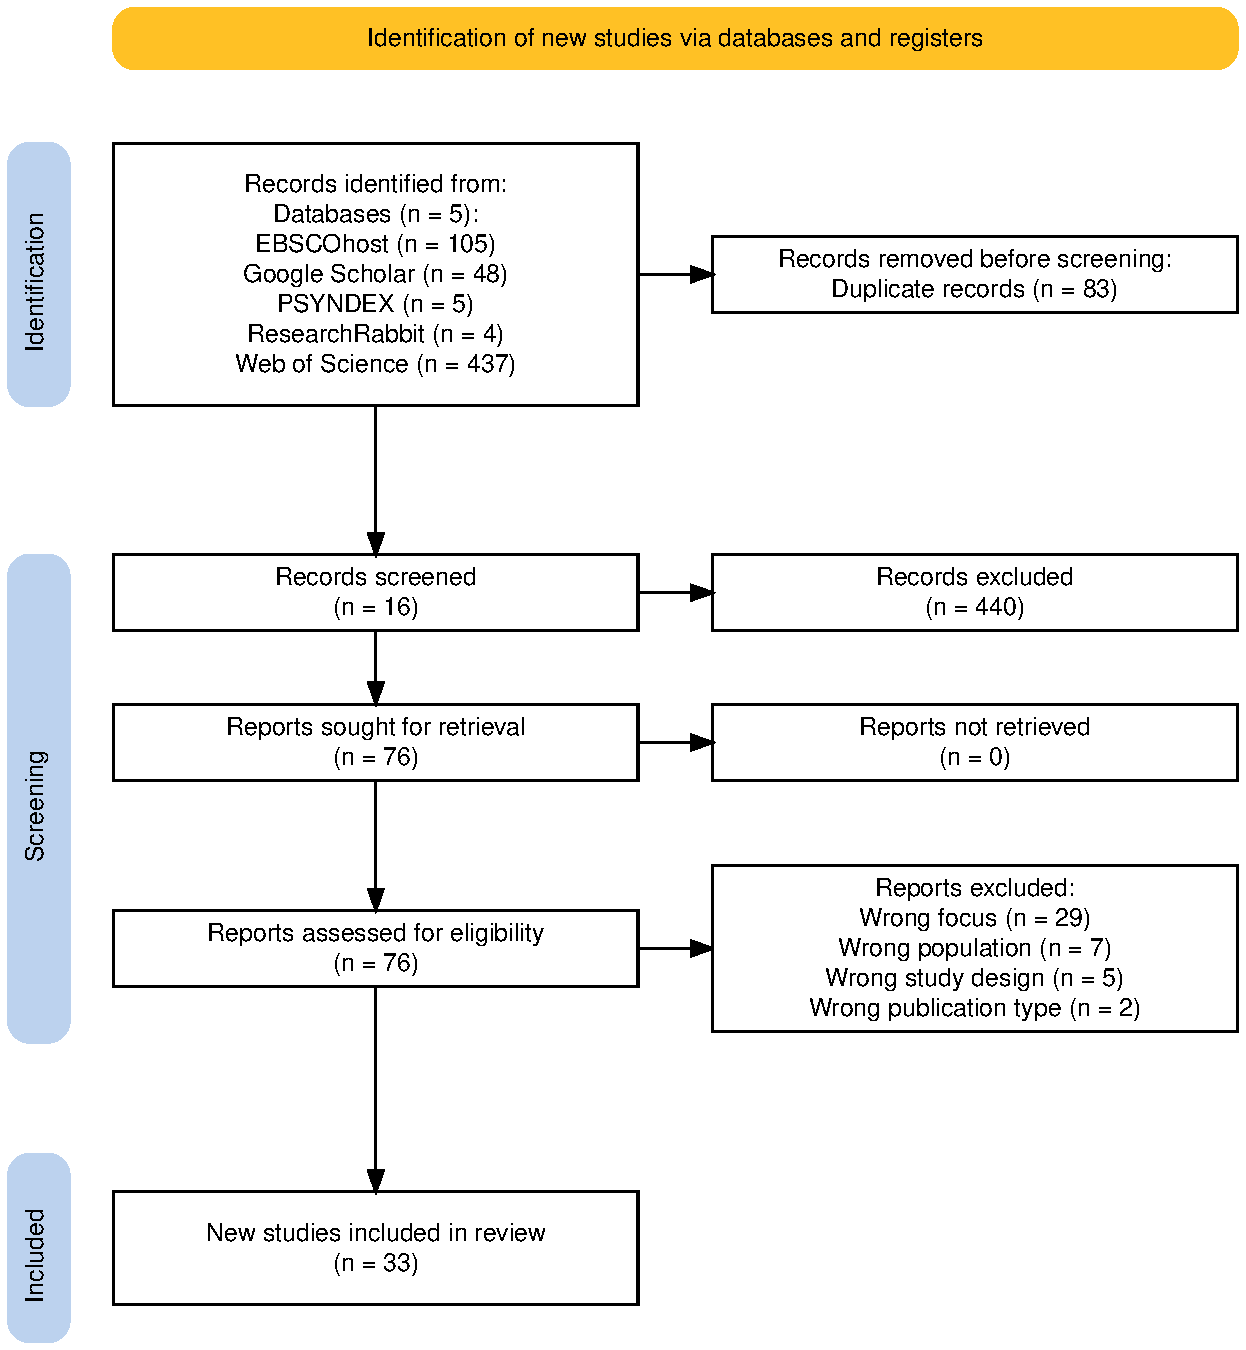
\includegraphics{files/prisma.pdf}
\caption{\label{fig:prisma}PRISMA flowchart of the screening process.}
\end{figure}

\subsection{R and RStudio}\label{r-and-rstudio}

THe following R packages were used to create this review: R (Version 4.4.1; R Core Team, 2024) and the R-packages \emph{citr} (Version 0.3.2; Aust, 2019), \emph{papaja} (Version 0.1.2.9000; Aust \& Barth, 2023), \emph{rmarkdown} (Version 2.27; Xie et al., 2018, 2020), and \emph{tinylabels} (Version 0.2.4; Barth, 2023)

\subsection{Participants}\label{participants}

\subsection{Material}\label{material}

\subsection{Procedure}\label{procedure}

\subsection{Data analysis}\label{data-analysis}

\section{Results}\label{results}

\section{Discussion}\label{discussion}

\newpage

\section{References}\label{references}

\phantomsection\label{refs}
\begin{CSLReferences}{1}{0}
\bibitem[\citeproctext]{ref-anthropicClaudeAiSonnet2024}
Anthropic. (2024). \emph{Claude {Ai} 3.5 {Sonnet}}. https://claude.ai/.

\bibitem[\citeproctext]{ref-R-citr}
Aust, F. (2019). \emph{Citr: 'RStudio' add-in to insert markdown citations}. \url{https://github.com/crsh/citr}

\bibitem[\citeproctext]{ref-R-papaja}
Aust, F., \& Barth, M. (2023). \emph{{papaja}: {Prepare} reproducible {APA} journal articles with {R Markdown}}. \url{https://github.com/crsh/papaja}

\bibitem[\citeproctext]{ref-R-tinylabels}
Barth, M. (2023). \emph{{tinylabels}: Lightweight variable labels}. \url{https://cran.r-project.org/package=tinylabels}

\bibitem[\citeproctext]{ref-githubGitHubCopilot2024}
GitHub, \& OpenAi. (2024). \emph{{GitHub Copilot}}. copilot.github.com.

\bibitem[\citeproctext]{ref-lakensImprovingYourStatistical2022}
Lakens, D. (2022). \emph{Improving {Your Statistical Inferences}}. Zenodo. \url{https://doi.org/10.5281/ZENODO.6409077}

\bibitem[\citeproctext]{ref-ouzzaniRayyanWebMobile2016}
Ouzzani, M., Hammady, H., Fedorowicz, Z., \& Elmagarmid, A. (2016). Rayyan---a web and mobile app for systematic reviews. \emph{Systematic Reviews}, \emph{5}(1), 210. \url{https://doi.org/10.1186/s13643-016-0384-4}

\bibitem[\citeproctext]{ref-positteamRStudioIntegratedDevelopment2024}
Posit team. (2024). \emph{{RStudio}: {Integrated} development environment for {R}} {[}Manual{]}. Posit Software, PBC.

\bibitem[\citeproctext]{ref-R-base}
R Core Team. (2024). \emph{R: A language and environment for statistical computing}. R Foundation for Statistical Computing. \url{https://www.R-project.org/}

\bibitem[\citeproctext]{ref-R-rmarkdown_a}
Xie, Y., Allaire, J. J., \& Grolemund, G. (2018). \emph{R markdown: The definitive guide}. Chapman; Hall/CRC. \url{https://bookdown.org/yihui/rmarkdown}

\bibitem[\citeproctext]{ref-R-rmarkdown_b}
Xie, Y., Dervieux, C., \& Riederer, E. (2020). \emph{R markdown cookbook}. Chapman; Hall/CRC. \url{https://bookdown.org/yihui/rmarkdown-cookbook}

\end{CSLReferences}


\clearpage
\renewcommand{\listfigurename}{Figure captions}

\clearpage
\renewcommand{\listtablename}{Table captions}


\end{document}
